\section{Methodology}

\begin{table}[]
    \caption{Notation Description}
    \centering
    \begin{tabular}{c|c}
    \hline
       $\mathbf{X}_{\alpha}$  & activity feature \\ \hline
       $\mathbf{X}_{\alpha}^{(i)}$ & $i^{th}$ feature group of activity feature \\ \hline
       $\mathbf{X}_{\beta}$  & user-specific feature \\ \hline
       $\mathbf{X}_{\gamma}$   & course-specific feature \\ \hline
       $\textbf{E}^{(i)}_\alpha$ & embedding of $\mathbf{X}_{\alpha}^{(i)}$ \\ \hline
       $\mathbf{E}_\beta$ & embedding of   $\mathbf{X}_{\beta}$ \\ \hline
        $\mathbf{E}_\gamma$ & embedding of   $\mathbf{X}_{\gamma}$ \\ \hline
         $\textbf{V}_\alpha$ &  activity feature maps \\ \hline
       $\mathbf{V}_\beta$ & user-specific feature map \\ \hline
        $\mathbf{V}_\gamma$ & course-specific feature map\\ \hline
    \end{tabular}
    \label{tab:my_label}
\end{table}

We now turn to discuss potential solutions to predict when and whether a user will drop out a specific course, 
by leveraging the patterns discovered in the above analysis. In summary, we propose an Attention-based Feature Interaction Network (AFIN) to deal with the dropout prediction problem. Different from previous work on this task. The proposed model incorporates context information, including course course correlation and user influence, into a unified framework. What's more, AFIN also adopts attention mechanism to learn the importance of different patterns for users with different context. 
Let us begin with a formulation of the problem we are going to address.

\subsection{Formulation}
	\label{ProblemDef}
	

\begin{figure}
	\centering
	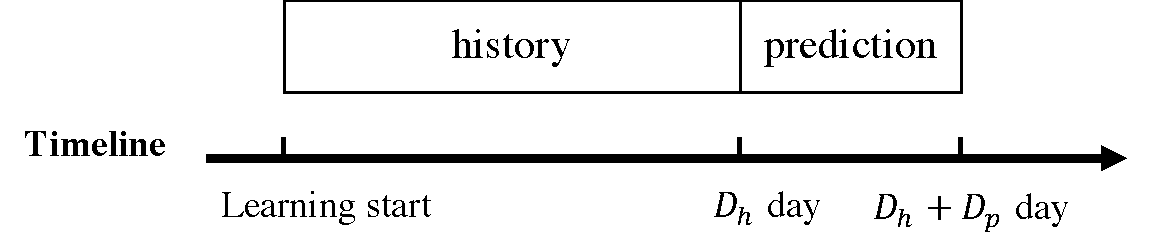
\includegraphics[width=\linewidth]{course-span.pdf}
	
	\caption{Dropout Prediction Problem. The first $D_h$ days are \emph{history period}, and the next $D_p$ days are \emph{prediction period}.}
	\label{fig:dataCons}
\end{figure}
\hide{
	\item{Activity Count/Ratio:} For each enrollment $(u,c)$, we calculate the number and ratio for each type of activities in table \ref{ResourceAction}. 
\item{Activity Temporal Statistics:} The whole duration time of a course is divided by weeks, and the activity counts and statistics(including \emph{max, min, stdev, median}) in different weeks are used as features.
\item{Activity Count in Hours Per Day:} We calculate user activity count for each hour in a day (24 hours).
\item{Activity Count in Day Per Week:} We compute user activity count for each day in a week (5 weekdays + 2 weekends).
\item{Activity N-gram Count/Ratio:} The N-grams of activity sequence is used to capture the correlations between neighbor activities. We employ N-gram activity count and ratio as the N-gram features.
\item{Engagement Style:} Following the taxonomy of engagement introduced by Anderson et al. \cite{Anderson:2014:EMO:2566486.2568042ß}, we use the $\emph{assignment fraction} = \frac{ \emph{watching video \#}}{ \emph{complete assignment \#}}$ to represent user's engagement pattern.
\item{Learning Time Span:} A user's learning time span is the duration between a user's first visit time and her last visit time on a course.  

\item{Effective Learning Time:} The \emph{effective learning time} introduced by Qiu et al. \cite{Qiu:2016:MPL:2835776.2835842} is an approximated method to compute user's actual study time on a certain course. This is calculated based on the time interval between user's \emph{watching video} and \emph{stop video}, and we employ this feature in our paper.

\item{Visiting Time Interval:} A user's interval time for visiting one course reflects user's interests in this course. The statistics(\emph{max, min, stdev, median}) of visiting time intervals are used as features.\\
}
\begin{table*}[]
	\caption{Activity Features}
	\centering
	\begin{tabular}{p{3.7cm}|p{13.4cm}}
		\hline
		Activity Count/Ratio  &  Total number and ratio of each type of learning activities\\ \hline
		Activity Temporal Statistics&  The whole duration time of a course is divided by weeks, and the activity counts and statistics(including \emph{max, min, stdev, median}) in different weeks are used as features.\\ \hline
		Activity Count Per Hour  &  The number of users' learning activities for each hour in a day (24 hours).\\ \hline
		Activity Count Per Day & The number of users' learning activities for each day in a week (5 weekdays + 2 weekends). \\ \hline
		Activity N-gram Count/Ratio & The N-grams of activity sequence is used to capture the correlations between neighbor activities. We employ N-gram activity count and ratio as the N-gram features. \\ 
	 \hline
		Engagement Style & Following the taxonomy of engagement introduced by Anderson et al. \cite{Anderson:2014:EMO:2566486.2568042ß}, we use the $\emph{assignment fraction} = \frac{ \emph{watching video \#}}{ \emph{complete assignment \#}}$ to represent user's engagement pattern.  \\ \hline
		Learning Time Span & A user's learning time span is the duration between a user's first visit time and her last visit time on a course.  \\ \hline
		Effective Learning Time & The \emph{effective learning time} introduced by Qiu et al. \cite{Qiu:2016:MPL:2835776.2835842} is an approximated method to compute user's actual study time on a certain course. This is calculated based on the time interval between user's \emph{watching video} and \emph{stop video}, and we employ this feature in our paper.\\ \hline
		Visiting Time Interval & A user's interval time for visiting one course reflects user's interests in this course. The statistics(\emph{max, min, stdev, median}) of visiting time intervals are used as features.
		\\ \hline
	\end{tabular}
	\label{tab:acvtityFeat}
\end{table*}

Our main task is to predict whether a user would dropout from an enrolled course in a pre-specified time window. In order to formulate this problem, we introduce the following definitions. \\


\emph{Definition 2.} \textbf{Enrollment Relation}:Let $\mathbb{C}$ denote the set of courses, $\mathbb{U}$ denote the set of users, and the pair $(u,c)$ denote user $u\in \mathbb{U}$ enrolls the course $c\in \mathbb{C}$.
The set of enrolled courses by $u$ is denoted as  $\mathbb{C}_u\subset \mathbb{C}$ and 
the set of users who have enrolled course $c$ is denoted as $\mathbb{U}_c\subset \mathbb{U}$.
We use $\mathbb{E}$ to denote the set of all enrollments, i.e., $\{(u,c)\}$\\


\emph{Definition 3.} \textbf{Learning Activity Vector}: 
In MOOCs, user $u$'s learning activities in a course $c$ can be formulated into a $m_x$-dimensional vector $\mathbf{X}(u,c) \in \mathbb{R}^{m_x}$, where each element of $\mathbf{X}$ is a pre-defined feature associated to user's learning activity in a course. Those features are extracted from user historical logs. The details are exhibited in Table \ref{tab:acvtityFeat}. \\

\emph{Definition 4.} \textbf{Context Information Vector}: Context information in MOOCs comprises user information and course information. User information is represented by user demographics (i.e. gender, age, location, education level) and user cluster (Cf. Section \ref{sec:temporal}). While course information is course category. Analogous to the learning activities, these context information is represented by a $m_z
$-dimensional vector $\mathbf{Z}(u,c) \in \mathbb{R}^{m_z}$ in this paper.  \\


%Activity pattern vector mainly includes users' learning behavioral features, which are extracted from user historical activity logs. The details are exhibited in Table \ref{tab:acvtityFeat}. User-related pattern vector consists of user demographics (i.e. gender, age, location, education level and user id) and user cluster (Cf. Section \ref{sec:temporal}). Course-related pattern vector,  including course id and course category, is used to represent course specific information in MOOCs. \\
%Specifically the pattern vector includes three types of patterns: activity pattern vector $\mathbf{X}_a \in \mathbb{R}^{m_a}$, user-specific pattern vector $\mathbf{X}_u \in \mathbb{R}^{m_u}$ and course-specific pattern vector $\mathbf{X}_c \in \mathbb{R}^{m_c}$.  

% into a paired tuple  $x = (a, t)$, where $a$ represents user's action(such as ``watching video'') and $t$ is the corresponding logged time stamp. In this paper, we focus on four types of learning activities: \emph{video, forum, assignment, web page}, which are described in table \ref{ResourceAction}. \\

%Each course has a set of available resources for users, such as video and forum. Here we use $R$ to represent the resource set of course on MOOCs. For each resource $r \in R$, there are a set of specific actions for it. We use $A$ to denote the action set. In this paper, we focus on four types of resources on MOOCs: \emph{video, forum, assignment, web page}, which are shown in table \ref{ResourceAction}, together with the corresponding actions. 

%Then a learning activity record of $u\in \mathbb{U}$ in one enrolled course $c\in \mathbb{U}_c$ at time $t$ can be represented as $X=(u,c,r,a,t)$, where $r\in R$ is the resource $u$ has accessed, $a\in A$ is the corresponding action on $r$. For each $(u,c) \in \mathbb{E}$, we use $\mathcal{X}_{uc}$ to represent user $u$'s historical learning activity set on $c$.\\

With these definitions, our problem of dropout prediction can be defined as: Given user $u$'s learning activity vector $\mathbf{X}(u,c)$ on course $c$ in \textit{history period} (as shown in Figure \ref{fig:dataCons}, it is the first $D_h$ days after the learning starting time), as well as her context information vector $\mathbf{Z}(u,c)$, our goal is to predict whether $u$ will drop out from $c$ in the \textit{prediction period} (as shown in Figure \ref{fig:dataCons}, it is the following $D_p$ days after \textit{history period}). More precisely, let $y_{(u,c)} \in \{0,1\}$ denote the ground truth of whether $u$ has dropped out, $y_{(u,c)}$ is positive if and only if $u$ has not taken activities on $c$ in the \textit{prediction period}. Then our task is to learn a function:
%Given user $u$'s activity sequence $X_{(u,c)}= [x_1, x_2,...,x_N]$ on course $c$ in \textit{history period}(as shown in Figure \ref{fig:dataCons}, it is the first $D_h$ days after the learning starting time), our goal is to predict whether $u$ will drop out from $c$ in the \textit{prediction period}(as shown in Figure \ref{fig:dataCons}, it is the following $D_p$ days after \textit{history period}). More precisely, let $y_{(u,c)} \in \{0,1\}$ denote the ground truth of whether $u$ has dropped out, $y_{(u,c)}$ is positive if and only if $u$ has not taken activities on $c$ in the \textit{prediction period}. Then our task is to learn a function:
$$f: (\mathbf{X}(u,c), \mathbf{Z}(u,c))\to y_{(u,c)}$$ \\

\hide{Let $\mathbb{C}$ denote the set of courses, $\mathbb{U}$ denote the set of users, and the pair $(u,c)$ denote user $u\in \mathbb{U}$ enrolls the course $c\in \mathbb{C}$.
The set of enrolled courses by $u$ is denoted as  $\mathbb{C}_u\subset \mathbb{C}$ and 
the set of users who have enrolled course $c$ is denoted as $\mathbb{U}_c\subset \mathbb{U}$.
We use $\mathbb{E}$ to denote the set of all enrollments, i.e., $\{(u,c)\}$.
Given this, our problem of dropout prediction can be defined as:}

\hide{
		\vspace{0.07in}
	   \emph{Definition 2.} \textbf{$t$-Dropout Prediction}: Given all users $\mathbb{U}$'s learning activity $\textbf{X}^t$ in all courses $\mathbb{C}$ before time $t$, our goal is to learn a function $f$ in order to infer
	   $$f: (\mathbb{U},\mathbb{C},\textbf{X}^t)\to \{y^t_{(u,c)}\}$$
	   \noindent where $y_{(u,c)} \in \{0,1\}$ indicates whether user $u$ would drop out ($y=1$) course $c$ 
	   after time $t$ or not. 
	   \vspace{0.07in}
}
\hide{
	   sequence $X_{(u,c)}= [x_1, x_2,...,x_N]$ on course $c$ in \textit{history period}(as shown in Figure \ref{fig:dataCons}, it is the first $D_h$ days after the learning starting time), our goal is to predict whether $u$ will drop out from $c$ in the \textit{prediction period}(as shown in Figure \ref{fig:dataCons}, it is the following $D_p$ days after \textit{history period}). More precisely, let $y_{(u,c)} \in \{0,1\}$ denote the ground truth of whether $u$ has dropped out, $y_{(u,c)}$ is positive if and only if $u$ has not taken activities on $c$ in the \textit{prediction period}. Then our task is to learn a function:
	 $$f: (u,c,X_{(u,c)})\to y_{(u,c)}$$
}    

	
\hide{
Based on the analyses in previous section, users' dropout in a course has high correlation with their context(similar courses and friends). How to construct a personalized prediction system for diverse users in MOOCs is a quite difficult problem. In this section, we introduce our methodology of personalized dropout prediction. We consider three types of features, i.e., activity features, user-related features and course-related features, when predicting users' dropout.
}
  \begin{table}
	\hspace{-0.01in}
	\centering
	\caption{Results of clustering analysis. C1-C5 --- Cluster 1 to 5; CAR --- average correct answer ratio. }
	\small
	\label{tab:sample}
	\setlength{\tabcolsep}{1mm}\begin{tabular}{@{}c@{}|l@{}|c|c}
		\hline
		\hline
		Category &  Type   & Conversational English Skills & Data Structure \\
		\hline
		\multirow{3}{*}{video}&  \#watch &74.80 & 32.48\\	
		\cline{2-4}
		& \#stop     &69.53 & 26.14\\
		\cline{2-4}
		& \#jump   &51.18 & 14.38\\
		\hline
		\multirow{2}{*}{forum}&  \#question & 0.049 & 0.038 \\
		\cline{2-4}
		& \#answer &1.10&0.12 \\
		\hline
		\multirow{2}{*}{assignment} & CAR &0.45 & 0.41 \\
		\cline{2-4}
		& \#revise  &0.09& 0.02 \\
		\hline
		\multirow{2}{*}{session}    & seconds &1,715 &714 \\
		\cline{2-4}                
		&  count     &3.61 &8.13 \\  
		\hline
		& dropout rate &0.74 &0.73 \\
		\hline	
		\hline
	\end{tabular}
	\normalsize
\end{table}
Please note that we define the prediction of dropouts for all users/courses together, as we need to consider the correlation between courses and influence between users. In next section, we will explain the motivations and details of our solution (Context-aware Feature Interaction Network) for this task.


%Another challenge we have to face is how to incorporate the course correlation and friend influence into the prediction. To solve these challenges, we proposed an Attention-based Feature Interaction Network (AFIN) to predict dropout by incorporating users' context information.
\subsection{Context-aware Feature Interaction Network}
\textbf{Motivation.} Based on the analyses results in Section \ref{sec:temporal}, we found that users' activity patterns in MOOCs highly depend on their context (e.g. course correlation and friends influence). However,  very few works have attempted to incorporate the context information into the dropout prediction framework.
 This is the main motivation for our approach: Context-aware Feature Interaction Network. 
 
 More specifically, we found the learning activity vector $\textbf{X}_a$ exhibits large differences across different courses and users, which would cause big bias in dropout prediction. Table \ref{tab:sample} presents an example of the average activity feature values on two courses (i.e. Conversational English Skills and Data Structure). We can observe that these features are totally different between two courses though they have a approximate user dropout rate. A general solution for this challenge is to augment the learning activity vector with its statistics of user-level and course-level and feed the augmented learning activity vector into the classifier directly. However, it always suffers from the curse of dimensionality and can not get a better performance. To tackle this issue, we employ convolutional neural networks (CNN) to learn a context-aware representation for each feature of learning activity vector by leveraging its statistics. This strategy is referred to context-smoothing in this paper. What's more, we also propose an attention mechanism to learn the importances of different activities by incorporating the context information into dropout prediction. Figure~\ref{fig:modelArch} shows the architecture of the proposed method.
 In the rest of this section, we will explain the context-smoothing and attention mechanism in details.
%The main technical contributions of Attention-based Feature Interaction Network (AFIN) lies in the proposal of context-smoothing and an attention mechanism to model the correlations among $\mathbf{X}_a$, $\mathbf{X}_u$ and $\mathbf{X}_c$.
%The idea of feature context-smoothing is to augment the context information into each feature and then use convolutional neural networks (CNN) to learn the representation of each feature. We also add an attention layer so as to learn the importances of activity patterns based on user-specific and course-specific patterns.

\textbf{Context-Smoothing.} The context-smoothing strategy has three steps: feature augmentation, embedding and feature fusion.
In feature augmentation, the learning activity vector $\mathbf{X}_a$ is expanded with its context statistics. 
\hide{
Specifically,  The context statistics of $i^{th}$ feature of $\mathbf{X}_a$ is defined by a mapping function from the original feature to several statistics over user and course, called user-specific context and course-specific context respectively:
\begin{equation}
\textbf{X}(u,c,i) =\left\{ \begin{aligned} 
f_s(\{X((\hat{u},c),i)|\hat{u}\in \mathbb{U}_c\}) \\
\oplus  \quad\quad\quad\quad\quad \\
f_s(\{X((u,\hat{c}),i)|\hat{c}\in \mathbb{C}_u\})   \\
\oplus  \quad\quad\quad\quad\quad \\
[X((u,c),i)]\quad \quad\quad\\
\end{aligned}\right.
\end{equation}
}
Specifically, for each original feature in $x_i(u,c) \in \textbf{X}(u,c)$,\footnote{We ommit the notation $(u,c)$ in the following description, if no ambiguity} we augment it with user-context statistics and course-context statistics. The user-context statistics of feature $x_i$ is defined by a mapping function $g_u(x_i)$ from the original feature to several statistics of $i^{th}$ feature over $u$, i.e., $g_u: x_i(u,c) \rightarrow [\text{avg}(\{x_i(u,*)\}), \text{max}(\{x_i(u,*)\}),\ldots]$. While course-context statistics are statistics over course represented by $g_c(x_i)$, analogously to $g_u$. We define $\mathbf{X}^{(i)}=[[x_i] \oplus g_u(x_i) \oplus g_c(x_i)]$ as the $i^{th}$ feature group of augmented activity feature.

%The user-specific context of feature $x_i$ is defined by a mapping function $g_u(x^{uc}_i)$ from the original feature to a context value defined over user $u$, e.g., 
%$g_u(x^{uc}_i) \rightarrow \text{avg}(\{x^{u.}_i\})$ indicates that a mapping to the average score of all the values of the $i^{th}$ feature associated with $u$.
\hide{
To deal with the sparsity problem, we first expand the original activity features with context information. The context information  is defined as the statistics of original features. 
For easy explanation, we can define 
$\hat{\mathbf{X}}(u,c)=[\textbf{X}((u,c),1),\textbf{X}((u,c),2),...,\textbf{X}{(u,c,m_a)}]$ to represent augmented activity feature vector, where each $\textbf{X}((u,c),i)\in \mathbb{R}^{m_g}$ is a feature group which consists of feature value $X((u,c),i)$ and its context:}
\hide{
\begin{equation}
    \textbf{X}(u,c,i) =\left\{ \begin{aligned} 
f_s(\{X((\hat{u},c),i)|\hat{u}\in \mathbb{U}_c\}) \\
 \oplus  \quad\quad\quad\quad\quad \\
   f_s(\{X((u,\hat{c}),i)|\hat{c}\in \mathbb{C}_u\})   \\
   \oplus  \quad\quad\quad\quad\quad \\
   [X((u,c),i)]\quad \quad\quad\\
\end{aligned}
\right
\end{equation}
}
\hide{
\begin{equation}
    \textbf{X}((u,c),i) =\left\{ \begin{aligned} 
f_s(  \mathbf{X}((*,c),i) ) \\
 \oplus  \quad\quad\\
   f_s( \mathbf{X}((u,*),i) )   \\
   \oplus  \quad\quad \\
   [X((u,c),i)]\quad \\
\end{aligned}
\right.
\end{equation}

\noindent where $f_s$ is a mapping function from a number set to its statistics: $f_s: \mathbb{X}\rightarrow [\text{avg}(\mathbb{X})), \text{max}(\mathbb{X}),...]$. $\oplus$ denotes concatenate operation between two vectors.   $\mathbf{X}((*,c),i)$ indicates the $i^{th}$ feature values of all users enrolled in $c$. While $\mathbf{X}((u,*),i)$ is the $i^{th}$ feature values over courses enrolled by $u$.}
%and course id, which are used to capture course specific information.

 The continuous features(e.g. activity features) can be simply represented by real numbers. While the categorical features(e.g. user id) are represented by a one-hot vector.
 
%For an enrollment $(u,c) \in \mathbb{E}$, we employ $\mathbf{Z}(u,c)=[Z^\alpha(u,c,1),Z(u,c,2),...,Z{(u,c,m_u)}]$ to represent activity feature vector, ,

We use $\mathbf{X}_\beta$
%=[X(u,1),X(u,2),...,X(u,m_u)]$ 
to denote the user-specific feature vector and $\mathbf{X}_\gamma$
%=[X(c,1),X(c,2),...,X(c,m_c)]$ 
to represent the course-specific feature vector. 
%These features are feed to an attention-based feature interaction network for dropout prediction. 
With the augmented features, we first learn the feature embedding and then use an CNN to learn feature representation (Cf. Figure~\ref{fig:modelArch}).

%\begin{algorithm}[H]
%\caption{Feature Augmentation}
%\begin{algorithmic}
%    \STATE \textbf{Input}: {activity feature $\mathbf{Z}^\alpha$, statistical function set $F$}\\
%    \STATE \textbf{Output}: {augmented activity feature $\hat{\mathbf{Z}}^\alpha(u,c)$} 
%    \FOR{$\mathbf{Z}^\alpha_{(u,c),i}$ in $\mathbf{Z}^\alpha(u,c)$}
%    \STATE compute user-specific statistical vector \mathbf{Z}^{s_u}_{(u,c),i}: $Z^{s_u}_{(u,c),i,j} = f_j(\{Z^{\alpha}_{u,\hat{c},v}|\hat{c} \in {C}_{u}\}),f_j\in F$ 
%    \STATE  
%    \ENDFOR
%\end{algorithmic}
%\end{algorithm}
%\begin{algorithm}[!h]
%	\caption{Feature Interaction.}  
%	\label{alg:Co-Training}  
%	\textbf{Input}: {activity feature $\mathbf{Z}^\alpha(u,c)$, user-related feature $\mathbf{Z}^\beta(u)$ and course-related feature $\mathbf{Z}^\gamma(c)$;}\\
%	\textbf{Output}: { dropout probability $\hat{y}_{(u,c)}$;}\\
%	\textbf{Step 1: Embedding}\\
%	Augment $\mathbf{Z}^\alpha(u,c)$ to $\hat{\mathbf{Z}}^\alpha(u,c)$, refers to ...} \\ 
%		\  Convert $\hat{\mathbf{Z}}^\alpha(u,c)$, $\mathbf{Z}^\beta(u)$ and $\mathbf{Z}^\gamma(c)$ to embedding representation. Refers to equation} \\
%	\textbf{Step2:Feature Fusion}\\
%	    \qquad compress  by a convolution layer.
%	    \qquad 
%\end{algorithm}

 \begin{figure}
 \hspace{-0.1in}
	\centering
	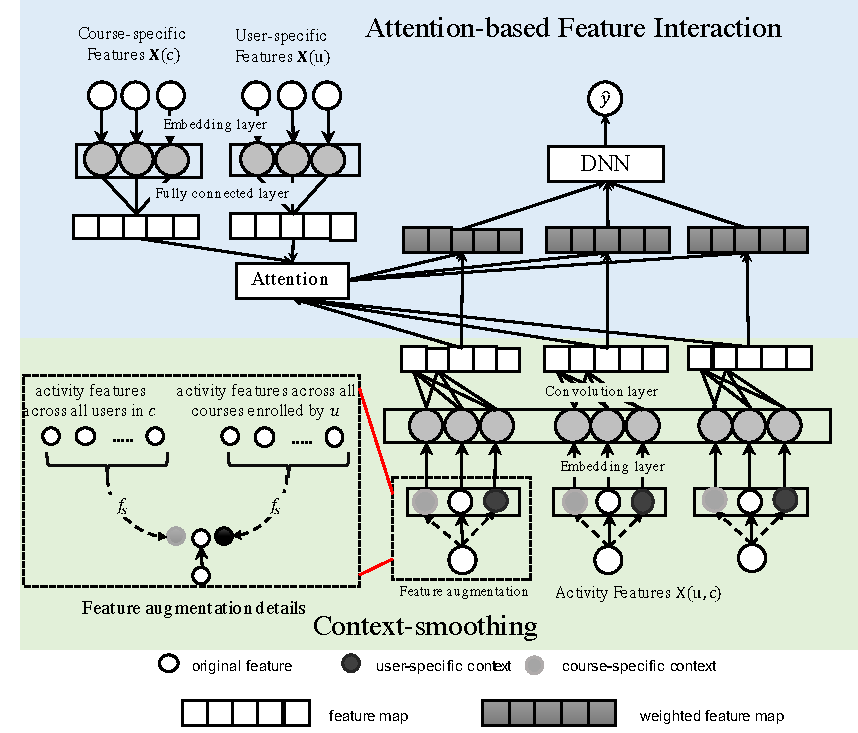
\includegraphics[width=\linewidth]{model_arch.pdf}
	
	\caption{The Architecture of Context-aware Feature Interaction Network.}
	\label{fig:modelArch}
\end{figure}


%\begin{algorithm}[t]
%\caption{Methodology}
%\begin{algorithmic}
 %   \STATE \textbf{Input}: {Activity feature $\mathbf{X}(u,c)$, user-related feature $\mathbf{X}(u)$ and course-related feature $\mathbf{X}(c)$}\\
  %  \STATE \textbf{Output}: {dropout probability $\hat{y}_{(u,c)}$

   % \STATE \textbf{Step1}: {Feature Context Smoothing}
    %\STATE\qquad (1). Augment the feature vector
    
%    \STATE\qquad (2). Augment $\mathbf{Z}^\alpha(u,c)$ to $\hat{\mathbf{Z}}^\alpha(u,c)$ and convert it to embedding matrix $\mathbf{E}^\alpha(u,c)$, refer to equation 3 to 5.
 %    \STATE \textbf{Step2}: {Feature Fusion}
  %   \STATE \qquad (1). Learning activity feature maps $\mathbf{V}^\alpha(u,c)$ from $\mathbf{E}^\alpha(u,c)$ by a convolution layer, refer to equation 6.
   %  \STATE\qquad (2). Learning user-related feature map $ \mathbf{V}^\beta(u)$ and course-related feature map $\mathbf{V}^\gamma(c)$ from $\mathbf{E}^\beta(u)$ and $\mathbf{E}^\gamma(c)$, refer to equation 7, 8.
     
%     \STATE \textbf{Step3}: {Attention-based Interaction}
 %    \STATE \qquad (1). Learning attention weights for activity feature maps, refer to equation 10.
  %   \STATE\qquad (2). Estimate $\hat{y}$ by feeding the weighted activity feature maps to DNN layer, refer to equation 12, 9.
% \end{algorithmic}
%\end{algorithm}


\hide{
\subsection{Attention-based Feature Interaction Network}
 We propose an attention-based feature interaction network(AFIN) to predict dropout probabilities for diverse users in MOOCs. The architecture of AFIN is illustrated in Figure \ref{fig:modelArch}. The model can learn users' preference for different activities by learning an attention weight for each activity feature. Specifically, the model consists of three major steps: \textit{Feature Embedding}, \textit{Feature Fusion} and \textit{Attention based Interaction}.
 incorporating user-specific information and course-specific information. 
}

%\vpara{Feature Embedding.}
Similar to most of deep learning methods, the first step of our model is to project each feature to a dense vector, which is called embedding. In our model, feature embedding matrix is simply obtained by multiplying the feature vector with a parameter matrix: 
%For user-specific feature and course-specific feature, we simply get their embedding by multiplying an matrix:
\begin{equation}
\mathbf{E} = \mathbf{X}\mathbf{W}_e
\end{equation}
where $\mathbf{E}$ is the feature embeddings, $X$ is the feature vector, $\mathbf{W}_e$ is parameter matrix. We use $\mathbf{E}_\beta$ to represent the user-specific feature embedding, $\mathbf{E}_\gamma$ to denote course-specific feature embedding and $\mathbf{E}_\alpha^{(i)}$ to represent the embedding of $i^{th}$ group of activity feature.
\hide{
\begin{equation}
    \mathbf{E}_\beta = \mathbf{X}_\beta\mathbf{W}^e_\beta
    \label{equ:u_emb}
\end{equation}
\begin{equation}
    \mathbf{E}_\gamma = \mathbf{X}_\gamma{W}^e_\gamma
    \label{equ:c_emb}
\end{equation}


\noindent where $\mathbf{E}_\beta \in \mathbb{R}^{m_\beta \times d_e}$ is user-specific embedding, $\mathbf{E}_\gamma \in \mathbb{R}^{m_\gamma \times d_e}$ is course-specific embedding; $\mathbf{W}^e_\beta \in \mathbb{R}^{m_\beta \times d_e}$ and $\mathbf{W}^e_\gamma \in \mathbb{R}^{m_\gamma \times d_e}$ are parameters. $m_\beta$ is the number of user-specific features and $m_\gamma$ is the number of course-specific features.
While for activity feature, each feature group is converted to the embedding group.
%
%Based on the analyses in Section?, a user's activities in a course are associated with her co-learning courses and co-learning users, 
%In this stage, we aims to incorporate users' context activity information into the prediction model by augmenting activity features. 
%Considering a user-course pair $(u,c) \in \mathbb{E}$, we first calculate the statistics,i.e., \textit{avg}, \textit{max} and \textit{stdev}, for all elements of $\mathbf{Z}^\alpha(u,c)$ across $u$'s co-learning users and her co-learning courses. By this way, we can obtain two associated vectors for each $Z^{\alpha}_{(u,c),i} \in \mathbf{Z}^\alpha(u,c)$, i.e., user-specific statistical vector $\mathbf{Z}^{s_u}_{(u,c),i}$ and course-specific statistical vector $\mathbf{Z}^{s_c}_{(u,c),i}$, of which each element is one of aforementioned statistical numbers: 
%\begin{equation}
%Z^{s_u}_{(u,c),i,j} = f_j(\{Z^{\alpha}_{u,\hat{c},v}|\hat{c} \in \mathbb{C}_{u}\}) 
%\end{equation}
%\begin{equation}
%Z^{s_c}_{(u,c),i,j} = f_j(\{Z^{\alpha}_{\hat{u},c,i}| \hat{u} \in %\mathbb{U}_c\})
%\end{equation}
%where $f_j \in \{avg, max, stdev\}$. $\mathbf{Z}^{s_c}_{(u,c),i}$ can be considered as the behavioral information summerized from all learners in the course, while $\mathbf{Z}^{s_u}_{(u,c),i}$ can be seen as user's general engagement habits in the MOOCs platform.
%Then these statistics are added into the activity feature. The augmented activity feature vector is denoted as 
%$\hat{\mathbf{Z}}^\alpha(u,c)$. $\hat{\mathbf{Z}}^\alpha(u,c)$ can be considered as the concatenate of $m_\alpha$ groups of vectors:
%$$\hat{\mathbf{Z}}^\alpha(u,c)=\hat{\mathbf{Z}}^\alpha_{(u,c), g_1} \oplus \hat{\mathbf{Z}}^\alpha_{(u,c), g_2}\oplus ...\oplus \hat{\mathbf{Z}}^\alpha_{(u,c), g_{m_\alpha}}\footnote{$\mathbf{a} \oplus \mathbf{b}$ denotes the concatenation between $\mathbf{a}$ and $\mathbf{b}$}$$ 
%Each group $\hat{\mathbf{Z}}^\alpha(u,c,g_i)\in \mathbb{R}^{m_g}$ is defined as the concatenate of the $i$-th original activity feature $Z^{\alpha}_{(u,c),i}$ and its two statistical vectors:
%$$\hat{\mathbf{Z}}^\alpha(u,c,g_i)=[Z^{\alpha}_{(u,c),i}]\oplus \mathbf{Z}^{s_u}_{(u,c),i} \oplus \mathbf{Z}^{s_c}_{(u,c),i}$$
%$$\hat{\mathbf{Z}}^\alpha_{(u,c),g_i} \in \mathbb{R}^{m_g}$$
The feature augmentation strategy is also illustrated in Figure \ref{fig:modelArch}. Then the augmented activity features $\hat{\mathbf{X}}(u,c)$ are fed into the embedding layer:
%Similar to other deep learning methods, we convert all features into a dense vector by:

\begin{equation}
\mathbf{E}^\alpha_i = \mathbf{X} \mathbf{W}^e_\alpha
\end{equation}

\noindent where $\mathbf{E}((u,c),i) \in \mathbb{R}^{{m_a} \times d_e}$is group embedding matrix of $\mathbf{X}((u,c),i)$;  $\mathbf{W}_a(i) \in \mathbb{R}^{m_a \times d_e}$ are parameters to learn.
}
%We denote the converted embedding representation of $\hat{\mathbf{Z}}^\alpha_{u,c,Field_i}$, $\mathbf{Z}^\beta(u)$,  $\mathbf{Z}^\gamma(c)$, as $\hat{\mathbf{E}}^\alpha_{u,c,Field_i} \in \mathbb{R}^{m_f \times d_e}$, $\mathbf{E}^\beta(u) \in \mathbb{R}^{m_\beta \times d_e}$ and $\mathbf{E}^\gamma(c) \in \mathbb{R}^{m_\gamma \times d_e}$ respectively,where $d_e$ is the dimension of embedding vector. 


%\subsubsection{Feature Fusion}
After projecting features into embedding vectors, the next step is to integrate the different features. We tackle it by applying a group-wise convolution operation on the group embeddings of activity features. The corresponding formula is as follows:

\begin{equation}
\mathbf{V}_\alpha^{(i)} = \sigma(\mathbf{W}_{\alpha} \delta (\mathbf{E}_\alpha^{(i)}+\mathbf{b}_\alpha) \footnote{$\delta (\mathbf{E})$ denotes flatting $\mathbf{E}$ to a vector}
\end{equation}

\noindent where $\mathbf{W}_{\alpha} \in \mathbb{R}^{d_f \times m_gd_e} $ and $\mathbf{b}_{\alpha} \in \mathbb{R}^{d_f}$ are parameters, $\sigma$ is activate function. $\mathbf{V}^{(i)}_\alpha \in \mathbb{R}^{d_f}$ is the $i^{th}$ group feature map of convolution layer. We should note that $\mathbf{W}_{\alpha}$ and $\mathbf{b}_\alpha$ share the same values across different groups. 
%Then all features in $ \hat{\mathbf{Z}}^\alpha (u,c)$ are converted $m_a$ feature maps:
%$\mathbf{V}^\alpha(u,c)= [\mathbf{V}^\alpha_{(u,c),1}, \mathbf{V}^\alpha_{(u,c),2},...,\mathbf{V}^\alpha_{u,c,m_\alpha}]$. 
This step can be considered as smoothing for the activity features. 
%This parameter sharing mechanism is similar to the convolutional layer in Convolutional Neural Network, and it is used to extract the local correlations between original features and corresponding context information. The feature fusion procedure can also be considered as context-aware normalization for activity features. 
Apart from activity features, user-specific features and course-specific features are compressed to two dense vectors by employing a fully connected layer:

\begin{equation}
\mathbf{V}_\beta = \sigma(\mathbf{W}_\beta \delta(\mathbf{E}_\beta) +\mathbf{b}_\beta)
\end{equation}
\begin{equation}
\mathbf{V}_\gamma = \sigma(\mathbf{W}_\gamma \delta(\mathbf{E}_\gamma) +\mathbf{b}_\gamma)
\end{equation}

\noindent where $\mathbf{W}_\beta \in \mathbb{R}^{d_f\times m_\beta d_e}$, $b_\beta \in \mathbb{R}^{d_f}$, $\mathbf{W}_\gamma \in \mathbb{R}^{d_f\times m_\gamma d_e}$, $b_\gamma \in \mathbb{R}^{d_f}$  are parameters. 
%$\mathbf{E}^\beta(u) \in \mathbb{R}^{m_\beta \times d_e}$ and  $\mathbf{E}^\gamma(c) \in \mathbb{R}^{m_\gamma \times d_e}$ are embedding matrices of user-context features and course-context features. 
$\mathbf{V}_\beta \in \mathbb{R}^{d_f}$ is user-specific feature map, while $\mathbf{V}_\gamma \in \mathbb{R}^{d_f}$ is course-specific feature map.

\subsubsection{Attention Mechanisms}
After learned the feature representations, we propose using attention mechanisms to incorporate user-specific features and course-specific features into the prediction model.
%The final step is to predict the dropout probability by modeling users' activity patterns. 
We can simple feed the activity feature map $\mathbf{V}_\alpha$ into an $L$-layer deep neural network(DNN) to learn the interactions of different activity features. Specifically, the input layer is the concatenate of $m_a$ feature maps in $\mathbf{V}_\alpha$. While each hidden layer can be formulated as:

\begin{equation}
\mathbf{V}_{d}^{(l+1)} = \sigma(\mathbf{W}_{d}^{(l)} \mathbf{V}_{d}^{(l)} + \mathbf{b}_{d}^{(l)} )
\end{equation}

\noindent where $l$ is the layer depth.  $\mathbf{W}_{d}^{(l)}$, $\mathbf{b}_{d}^{(l)}$ are model parameters. $\mathbf{V}_{d}^{(l)} $ is output of $l$-layer. The final layer a sigmoid function which used to estimate the dropout rate. By this way, the model can capture the high-order interactions of different kinds of activities. However, based on the cluster analysis in previous section, MOOCs learners always exhibit different engagement habits, which the single DNN model can not capture. To tackle this problem, we adopt the attention mechanism to model users' preference for different activities. The basic idea is to learn an attention weight for each vector in $\mathbf{V}_\alpha$ based on $\mathbf{V}_\beta$ and $\mathbf{V}_\gamma $: 

\begin{equation}
\lambda_i = Softmax(\mathbf{W}_\lambda(\mathbf{V}_\beta \oplus \mathbf{V}_\gamma \oplus  \mathbf{V}_\alpha^{(i)}) + b_\lambda)
\end{equation}

\noindent where $\lambda_i$ is the attention weight of $i^{th}$ vector, it can also be seen as the importance of the $i^{th}$ feature in $\mathbf{X}(u,c)$. Finally, we feed the concatenate of weighted feature maps into DNN for the dropout prediction:

\begin{equation}
\hat{y} = f_{DNN}(\mathbf{\lambda}\mathbf{V}_\alpha)
\end{equation}

\noindent where $\hat{y}_{(u,c)} \in [0,1]$ denotes the probability of $u$ dropping out from course $c$.
All the parameters can be learned by minimizing the follow objective function:

\begin{equation}
\begin{split}
L(\mathbf{\Theta}) =  &-\sum_{(u,c)\in \mathbb{E}} [y_{(u,c)}\log(\hat{y}_{(u,c)}) \\
             &+(1-y_{(u,c)})\log(1-\hat{y}_{(u,c)})]
\end{split}
\end{equation}

\noindent where $\mathbf{\Theta}$ denotes the set of model parameters, $y_{(u,c)}$ is the corresponding ground truth, $\mathbb{E}$ is the set of all enrollments.



\subsection{Model Ensemble}
\label{sec:ensem}
For further improving the prediction performance, we also design an ensemble learning strategy by combining AFIN with the XGBoost \cite{Chen:2016:XST:2939672.2939785}, one of the most effective gradient boosting framework. Specifically, we obtained the output vector of DNN's $(L-1)^{th}$ layer, which is denoted by $\mathbf{V}_{d}^{(L-1)}$, from the successfully trained AFIN and use it as features to train a XGBoost. The original features ,i.e., augmented activity features, user-specific features and course-specific features are also fed to the XGBoost. This strategy is a little like stacking \cite{wolpert1992stacked}, but the difference is that the latter is to feed one model's predict probability to another one.
s